\chapter{The Nitrogen-Vacancy center in Diamond}
\label{controlingspinsindiamond}

%Write abstract of chapter

%Introduce definition of system.

\section{Initialization and readout of the electronic-spin state}

\begin{figure}[htbp]
    \centering
    \begin{subfigure}[t]{0.49\textwidth}\centering
        \caption{}
        \label{fig:Sil_Robledo}
        \includegraphics{Img/Sil_Robledo.pdf}
    \end{subfigure}
    \begin{subfigure}[t]{0.49\textwidth}\centering
       \caption{}
       \label{fig:readoutRobledo}
       \includegraphics{Img/readout_Robledo.pdf}
   \end{subfigure}
   \caption{\Cref{fig:Sil_Robledo}, Sil. \Cref{fig:readoutRobledo}. }
\end{figure}
\section{Controlling the electronic-spin state}
\label{spincontrol}

The electronic ground state Hamiltonian can be written as\citep{Bernien2014Control}:
 \begin{equation}
H_\mathrm{GS} = \Delta {S_\mathrm{z}}^2 + \gamma_e \mathbf{B} \cdot \mathbf{S}
\end{equation}

With zero field splitting $\Delta \approx 2.88 \mathrm{GHz}$  and gyro-magnetic ratio $\gamma_e  = 2.802$ MHz/G . In this expression the interactions with the nitrogen nucleus and the carbon spin bath are not included. By applying a magnetic field $B_\mathrm{z}$ along the NV-axis the degeneracy of the  $m_s =\pm1$ states is lifted by the Zeeman effect. We define our electronic qubit  by the two level system with  $m_s=0:=|0\rangle$ and $m_s = +1 := |1\rangle$.

On the Bloch-sphere the state vector rotates around the quantization-axis with a frequency depending on the energy splitting between the two states; the Larmor frequency.
For the NV-electronic spin transition used the Larmor frequency is given by \cref{eq:larmor_electronic_spin}.
\begin{equation}
    \omega_L =\Delta + \gamma_e {B_\mathrm{z}}
    \label{eq:larmor_electronic_spin}
\end{equation}

By applying an external field a term is effectively added to the Hamiltonian, changing the quantization-axis and thereby its evolution. By applying microwaves with the right frequency this can be used to selectively drive the transition from the  $|0\rangle$ state to the $|1\rangle$ state\citep{Jelezko2004Observation}.


\section{Controlling nuclear spins}


\subsection{The Hyperfine Interaction}
The coupling between the NV-centers electronic spin and a nuclear-spin is given by the hyperfine-interaction. The hyperfine-interaction is a spin dependent interaction that is not present for spin-0 particles such as carbon-12.

For nuclear spins the Hamiltonian depends on the electronic spin-state of the NV-center.
For a magnetic field ($B_\mathrm{z}$) in the z-direction the Hamiltonian is given by \cref{eq:nuclear_hamiltonian_0} when the electronic-spin is in the $m_s = 0$ state, and by \cref{eq:nuclear_hamiltonian_1} when in the $m_s = +1$ state\citep{Taminiau2014Universal}. Where $\gamma_n$ is the gyro-magnetic ratio of the nucleus.
 \begin{equation}
 \label{eq:nuclear_hamiltonian_0}
H_0= \gamma_{n} B_\mathrm{z} I_\mathrm{z}
\end{equation}
\begin{equation}
 \label{eq:nuclear_hamiltonian_1}
    H_1 = \gamma_{n} B_\mathrm{z} I_\mathrm{z} +H_{\mathrm{HF}}
\end{equation}

The Larmor frequency for a nucleus is given by  \cref{eq:nuclear_larmor}.
\begin{equation}
\label{eq:nuclear_larmor}
\bm{\omega_L} = \gamma_{n}B_\mathrm{z} \cdot\bm{\hat{\mathrm{z}}}
\end{equation}

The hyperfine ($H_{\mathrm{HF}}$) term consists of a contact term and a dipole term.
The contact term results from an overlap between the electronic- and nuclear- wave-functions making it negligible for all but the nuclear-spins closest to the NV-center.

\begin{figure}[htbp]
\centering
    \begin{tikzpicture}
        \node[anchor=south west,inner sep=0] at (0,0) {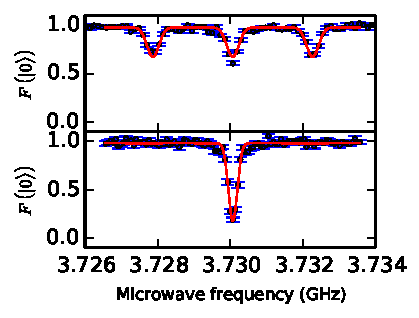
\includegraphics{Img/DarkESR_2.pdf}};
        \node (A) at (2.6,4.4) {};
        \node (B) at (3.92,4.4) { };
        \node (C) at (5.3,4.4) { };
        \draw[latex-latex, font=\small] (A) -- node[label =270: $A_\mathrm{N}$] {} (B);
        \draw[latex-latex, font=\small] (B) -- node[label =270: $A_\mathrm{N}$] {} (C);
    \end{tikzpicture}
    \caption{ Electron Spin Resonance (ESR) for uninitialized (top) and initialized nitrogen spin (bottom) of the $m_s =0 \rightarrow m_s = +1$ transition. In a dark ESR the spin is prepared in $\ket{0}$, a microwave pulse is applied and then the $\ket{0}$ state is read-out again. This is done for a range of frequencies. When the microwave is on resonance with a transition the spin will be rotated and a dip will be visible in the signal. In the top figure the transition is split due to the interaction with the nearby nitrogen atom. In the lower figure the nitrogen state is initialized and the splitting disappears.}
    \label{fig:HF_split_levels}
\end{figure}

\subsection{Strongly-coupled spins}
An example of a strongly coupled spin is the NV-nitrogen spin.
The strength of the coupling between the nitrogen and the electronic spin is $A_\mathrm{N} = 2\pi \cdot 2.186\quad \mathrm{MHz} $\citep{Bernien2014Control} and it acts along the NV-axis.
\Cref{fig:HF_split_levels} clearly shows the $m_s =0 \rightarrow m_s=+1$ transitions being split due to hyperfine-coupling to the nitrogen.
This splitting can be used to control the nitrogen.
By first initializing in the $m_s =+1$-state and then applying a slow pulse that turns only one of the three nitrogen spin-states back to $m_s=0$ and reading out the nitrogen-spin can be initialized. By only continuing on a positive outcome the spin is initialized in the state that was rotated back to $m_s =0$. We call this measurement-based-initialization (MBI).
The lower panel of \cref{fig:HF_split_levels} shows a Electron-Spin-Resonance (ESR) after nitrogen-MBI.

In a similar way strongly-coupled carbon-13 atoms can be controlled\citep{Robledo2011HighFidelity}.
For most strongly-coupled carbons the contact term in the hyperfine is not negligible.
For these carbons hyperfine couplings have been measured\citep{Smeltzer201113} and calculated\citep{Gali2008Ab,Gali2009Identification}.

\subsection{Decoherence}


When addressing a spin qubit we usually drive transitions between energy levels.
When the electronic-spin couples to a nuclear-spin these energy levels are shifted depending on the state of the nucleus.
In this way each spin has an individual back-action on the electronic-spin.

Most of these spins only shift the spin by a tiny amount making it hard to distinguish them from each other.
Because the states of these spins fluctuate the transitions of the NV-center are continuously shifting around, effectively causing a broadening of the transitions.
We call these very-weakly-coupled spins the spin-bath.

If the coupling between a spin and the NV-center is strong enough it is possible to resolve and address its transitions.
Transitions between energy levels can be resolved if the difference between them is larger than the width of the transition.

How narrow a transition is is related to how accurately it can be addressed.
The largest variations in the spin-bath, that determine the position of the transition, occur between experiments.
!
Need to add some sentences here about why T2 star is measurement for this
!
The time before a transition shifts out of resonance, or a signal decoheres, is usually expressed by $T_2^*$ and is measured by a Ramsey experiment, see \cref{fig:Ramsey_gijs}.

\begin{figure}[htbp]
    \centering
    \begin{subfigure}[t]{0.49\textwidth}\centering
        \caption{}
        \includegraphics{Img/Ramsey_Gijs.pdf}
        \label{fig:Ramsey_gijs}
    \end{subfigure}
    \begin{subfigure}[t]{0.49\textwidth}\centering
        \caption{}
        \includegraphics{Img/electron_T2star.pdf}
        \label{fig:electron_T2*}
    \end{subfigure}
        \caption{
        \Cref{fig:Ramsey_gijs}, schematic representation of a Ramsey experiment. Figure from \citet{Lange2012Quantum}.
        In a Ramsey experiment a qubit is initialized along the z-axis before being subjected to a $\pi/2$-pulse that moves it into the XY-plane of the Bloch-sphere.
        It freely evolves for a time $\tau$ before being subjected to a final $\pi/2$ pulse and read out along the z-direction.
        By applying a detuning to the rotating frame the spin will pick up a phase $\phi = \omega_d \tau$ during free evolution.
        The final pulse will rotate the spin towards the poles depending on the phase picked up during free evolution.
        This manifests itself as an oscillation.
        Because the configuration of the spin-bath is slightly different from experiment to experiment the frequency of the oscillation will vary from repetition to repetition.
        \Cref{fig:electron_T2*} shows a Ramsey experiment for the electronic spin.
        A $T_{2,e}^*$ of $4.54 \pm 0.14 \mu\mathrm{s}$ was measured for the electronic spin. The decay follows a Gaussian profile within uncertainty $n = 1.81 \pm 0.14$. }
\end{figure}

The decay of the amplitude $K$ in an electron Ramsey experiment is given by \cref{eq:Ramsey_decay}.
\begin{equation}
    K(\tau) = e^{-(\tfrac{\tau}{T_{2e}^*})^2}
    \label{eq:Ramsey_decay}
\end{equation}
We define $T_{2e}^*$ as the $1/e$ value of the Gaussian decay. The Electron-Spin-Resonance (ESR)\footnote{See \cref{fig:HF_split_levels} for an example of a dark ESR.} frequency spectrum for negligible power broadening is given by the Fourier transform of \cref{eq:Ramsey_decay}. Where $\omega = 2\pi \cdot f$\footnote{For clarity the factor of $2\pi$ is stated explicitly throughout this thesis to distinguish real and angular frequency. }.
\begin{equation}
    \mathcal{F} \{ K(\tau) \} =  T_2^* \sqrt{\pi} e^{-\tfrac{(2\pi \cdot f) ^2 \cdot T_{2e}^{*2}}{ 4}}
\end{equation}
Two identical Gaussians can be readily resolved if the separation between their maxima is larger than their full-width-half-maximum (FWHM).
The FWHM of the dark ESR is given by \cref{eq:FWHM}.
\begin{equation}
    2\pi \cdot \mathrm{FWHM} = 2\pi \cdot \frac{2\sqrt{\ln{2}}}{\pi T_{2e}^*}
    \label{eq:FWHM}
\end{equation}

\subsection{Definition of strongly coupled }
We define a spin to be strongly coupled when it is possible to readily resolve its transition.

An estimation of when spins can be resolved can be made by looking at the strength of the hyperfine interaction.
The splitting caused by a carbon spin is equal to twice the total interaction strength $A$ at low magnetic field ($\gamma_e B \ll A$). In the limit of high magnetic field ($\gamma_e B \gg A$) only the parallel component of the interaction $A_\parallel$ contributes to the splitting.
We can readily resolve a transition when the shift due to the corresponding interaction is larger than the FWHM of the transition.

\begin{align}
     2\pi \cdot |\bm{A}|\gg 2\pi \cdot \frac{\sqrt{\ln{2}}}{\pi T_{2e}^*} , \quad \mathrm{for } \quad \gamma_e B \ll A  \\
     2\pi \cdot A_\parallel \gg 2\pi \cdot \frac{\sqrt{\ln{2}}}{\pi T_{2e}^*}, \quad \mathrm{for } \quad \gamma_e B \gg A
     \label{eq:def_strongly_coupled}
 \end{align}

NV-centers have a typical electron $T_{2e}^* \approx 2\mu \mathrm{s}$\footnote{At a natural concentration of $1.1 \%$ carbon-13.} that depends on the exact configuration of the spin-environment.
On the sample used for the experiments $T_{2,e}^* = 4.54 \pm 14 \mu\mathrm{s}$ was measured, see \cref{fig:electron_T2*}.
Increasing the carbon-13 concentration generally reduces $T_{2e}^*$.
For a typical NV-center this means that the coupling between the carbon and the NV-center must be larger than $2\pi\cdot$130kHz for the carbon to be directly addressable for a typical NV-center and larger than $2\pi\cdot$ 58kHz for our sample.



























































% ------------------------------------------------------------
% ------------------------------------------------------------
% ------------------------------------------------------------


% % TODO_MAR: Rewrite introduction of diamond spin control chapter

% %Explain here how general experiment looks
% \section{OLD CHAPTER NV }
% It has been shown that the nuclear- and electron- spin-state of the NV- center can be initialized, controlled and read-out using microwave- and laser- pulses\citep{Robledo2011HighFidelity}. In these experiments two lasers that are resonant with transitions in the NV- center are used to initialize the electronic spin state.
% One of these two lasers is used to read out the electronic spin state and an off-resonant laser is used to reset the system. Microwaves are used to drive transitions between the different nuclear and electronic spin states.
% %Add figure explaining read out en init.

% Strongly coupled nuclear spins can be initialized by conditionally rotating the electronic state to a state that is read out only if the Carbon is in the desired state, when the electronic state readout has a positive result the system is projected into the desired state. We call this Measurement Based Initialization (MBI).
% %
% %
% %%%%%%%%%%%%%%%%%%%
% %TODO_MAR: add picture of Sil, schematic (with laser only hits one line)
% %%%%%%%%%%%%%%%%%%%
% %
% %
% % Explain pump laser and excitation laser,
% % Explain experiment starts with checking if Lasers are on resonance
% % Explain Nitrogen initialization to remove term from the Hamiltonian
% %
% % Explain structure of typical experiment and experimental setup
% % Setup, same as in old papers. State temperature 4K, state that magnetic field is used.
% %Structure.
% %CR-check , Init electron with lasers, Init Nitrogen, do fancy pulse sequence, readout, possibly feed forward, more pulses, RO again.
% %
% Our experiments are build around the same basic tools\comment{As the Robledo experiment? }.
% Each experiment starts with a Charge-Resonance check \comment{Explain how CR-Check works? Ref?}that verifies if the lasers are still on resonance.
% After that the Nitrogen spin state is initialized using MBI.\comment{In what state is the Nitrogen initialized?}
% Once the system is initialized the actual experiment is performed.
% An experiment consists of one or multiple blocks of microwave pulses and optical readouts.

% All experiments were performed on a custom-build cryostat setup operating at liquid helium temperatures described in detail in \citet[chap.~3]{Bernien2014Control}. The setup was additionally outfitted with a movable neodymium magnet that applied a magnetic field of ~300G to the sample.



% % \section{Dynamical decoupling}
% % DONT need to explain general dynamical decoupling?
% %Explain what dynamical decoupling is, decoupling from environment by 'inverting' the enviroment thus reducing influence of decoherence causing carbons.
% %Show figure from Tim's paper showing extended electron coherence times.
% % Make bridge to next chapter by refering paper again showing that it's possible to control carbons in this way by resonantly doing this
